\PassOptionsToPackage{unicode}{hyperref}
\documentclass[
  ukrainian,
  14pt
]{extreport}
\usepackage{lmodern}
\usepackage{hyperref}
\makeatletter
\hypersetup{
    colorlinks=true,
    linkcolor=blue,
    filecolor=magenta,
    urlcolor=cyan,
}
\makeatother
\usepackage{amssymb,amsmath,amsthm,url}
\usepackage[margin=2cm]{geometry}
\usepackage{longtable,booktabs}
\usepackage{etoolbox}
\usepackage{titling}
\usepackage{graphicx}
\usepackage{float}
\usepackage[dvipsnames]{xcolor}
\usepackage[ukrainian]{babel}
\usepackage{setspace}
\usepackage{xcolor}
\usepackage{multirow}
\usepackage{comment}
\usepackage{booktabs}
\usepackage{tikz}
\setcounter{secnumdepth}{-1} 
\usepackage{unicode-math}
  \defaultfontfeatures{Scale=MatchLowercase}
  \defaultfontfeatures[\rmfamily]{Ligatures=TeX,Scale=1}
  \setmainfont[]{Times New Roman}
  \setsansfont[]{Arial}
  \setmonofont[]{Consolas}
  \makeatother
\usepackage[labelsep=period]{caption}
\usepackage{subcaption}

\author{}
\title{\Huge Лабораторна робота №6 \\\Large Підсилювачі на транзисторах}
\date{}
             
\begin{document}
\begin{titlepage} 
	\newcommand{\HRule}{\rule{\linewidth}{0.5mm}} 
	
	\center 
	
	\textsc{\Large МІНІСТЕРСТВО ОСВІТИ І НАУКИ УКРАЇНИ\\ \Large КИЇВСЬКИЙ НАЦІОНАЛЬНИЙ УНІВЕРСИТЕТ ІМЕНІ ТАРАСА ШЕВЧЕНКА}\\[1.5cm] 

	
	\HRule\\[0.4cm]
	
	{\huge \bfseries  Лабораторна робота №6 \\\Large \bfseries 
    Операційні підсилювачі з негативним зворотним зв'язком
    }\\[0.4cm]
	
	\HRule\\[1.5cm]

	
	

	{\large\textit{Автор}}\\
	\large Столяров Андрій Дмитрович, \\\large група 5-А, Фізичний Факультет 
	
	
	\vfill\vfill\vfill 
	\vfill
	{\normalsize Київ, \today} 
\end{titlepage}
\tableofcontents
\clearpage
\section{Вступ}
Об'єкт досдіження — ОП, їхні ВАХ.

\subsection{Мета}
Ознайомитися з властивостями операційних
підсилювачів, опанувати способи підсилення електричних сигналів схемами з
ОП, охопленим негативним зворотним зв'язком та способи виконання
математичних операцій за допомогою схем з ОП.

\subsection{Методи дослідження}
це метод співставлення: одночасне спостереження вхідного та вихідного
сигналів на екрані двоканального осцилографа із наступним вимірюванням і
порівнянням їх параметрів.


\section{Теоретичні відомості}
\subsection{Терміни і означення}
\textbf{Операційний підсилювач} — це диференціальний підсилювач постійного
струму, який в ідеалі має нескінченний коефіцієнт підсилення за напругою і
нульову вихідну напругу за відсутності сигналу на вході, великий вхідний опір
і малий вихідний, а також необмежену смугу частот підсилюваних сигналів.

Раніше такі високоякісні підсилювачі використовувалися виключно в
аналогових обчислювальних пристроях для виконання математичних
операцій, наприклад, складання та інтегрування. Звідси і походить їх назва –
операційні підсилювачі (ОП).

Створення зворотного зв'язку полягає в тому, що частина вихідного
сигналу підсилювача повертається через ланку зворотного зв'язку (ЗЗ) на
його вхід. Якщо сигнал зворотного зв'язку подається на вхід у протифазі до
вхідного сигналу (різниця фаз $\Phi = 180^\circ$ ), то зворотний зв'язок називають
негативним (НЗЗ). Якщо ж він подається на вхід у фазі до вхідного сигналу
($\Phi = 0^\circ$), то такий зворотний зв'язок називають позитивним (ПЗЗ).
\subsection{ОП як інтегральна мікросхема}
У сучасній електроніці для конструювання різних електронних пристроїв
(підсилювачів, детекторів, перетворювачів і т. д.) використовуються інтегральні
мікросхеми. Шляхом комутації (створення певних електричних з'єднань) виводів
інтегральних мікросхем і додавання кількох зовнішніх дискретних елементів
(резисторів, конденсаторів, діодів і т. п.) вдається створити великий набір
різноманітних електронних схем на основі одієї і тієї ж мікросхеми.
Основною інтегральною мікросхемою для створення аналогових електронних
пристроїв є операційний підсилювач (ОП). ОП являє собою мікросхему, що за
своїми розмірами і ціною практично не відрізняється від окремого транзистора,
хоча вона й містить кілька десятків транзисторів, діодів і резисторів.
Завдяки практично ідеальним характеристикам ОП реалізація на їх основі різних
схем виявляєьться значно простішою і дешевшою, ніж на окремих транзисторах
і резисторах.
Операційним підсилювачем називають багатокаскадний диференціальний
підсилювач постійного струму, який має в діапазоні частот до кількох десятків
кілогерц коефіцієнт підсилення більший за 104 і за своїми властивостями
наближається до уявного «ідеального» підсилювача. Під ``ідеальним'' розуміють
такий підсилювач, який має:
\begin{enumerate}
    \item нескінченний коефіцієнт підсилення за напругою диференціального вхідного
    сигналу ($K \rightarrow \infty$);
    \item нескінченний вхідний імпеданс ($Z_{in} \rightarrow \infty$);
    \item нульовий вихідний імпеданс ($Z_{out} \rightarrow \infty$);
    \item  рівну нулеві напругу на виході ($U_{out} = 0$) при рівності напруг на вході
    ($U_{in_{1}} = U_{in_{2}}$) ;
    \item нескінченний діапазон робочих частот.
\end{enumerate}

Характеристики реального ОП не такі ідеальні, як хотілося б. Однак, для
практичних цілей ці характеристики близькі до ідеальних: коефіцієнт підсилення
для низьких частот (за постійним струмом) $K > 10^4$; вхідний опір $R_{in} > 10^6$ Ом;
вихідний опір $R{out} < 10^2$ Ом; коефіцієнт підсилення падає до 1 на частоті
порядка $10^6$ Гц (1 МГц); напруга зміщення $U3$ (визначається як напруга, яку
потрібно подати на вхід ОП, щоб вихідна напруга стала рівною нулеві) для
більшості ОП не перевищує 10 мВ, а для прецизійних – 10 мкВ.
Прототипом ОП може слугувати класичний диференціальний підсилювач з
двома входами і несиметричним виходом.

\section{Хід Роботи}
\subsection{Інвертувальний підсилювач}
\begin{figure}[H]
    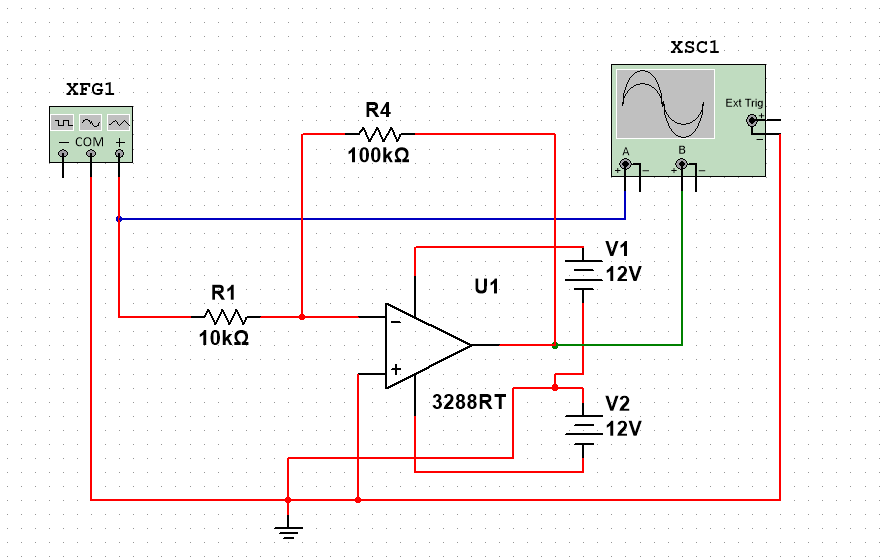
\includegraphics[width=0.6\textwidth]{imgs/1-1.png}
    \centering
    \caption{Схема}
\end{figure}
\begin{figure}[H]
    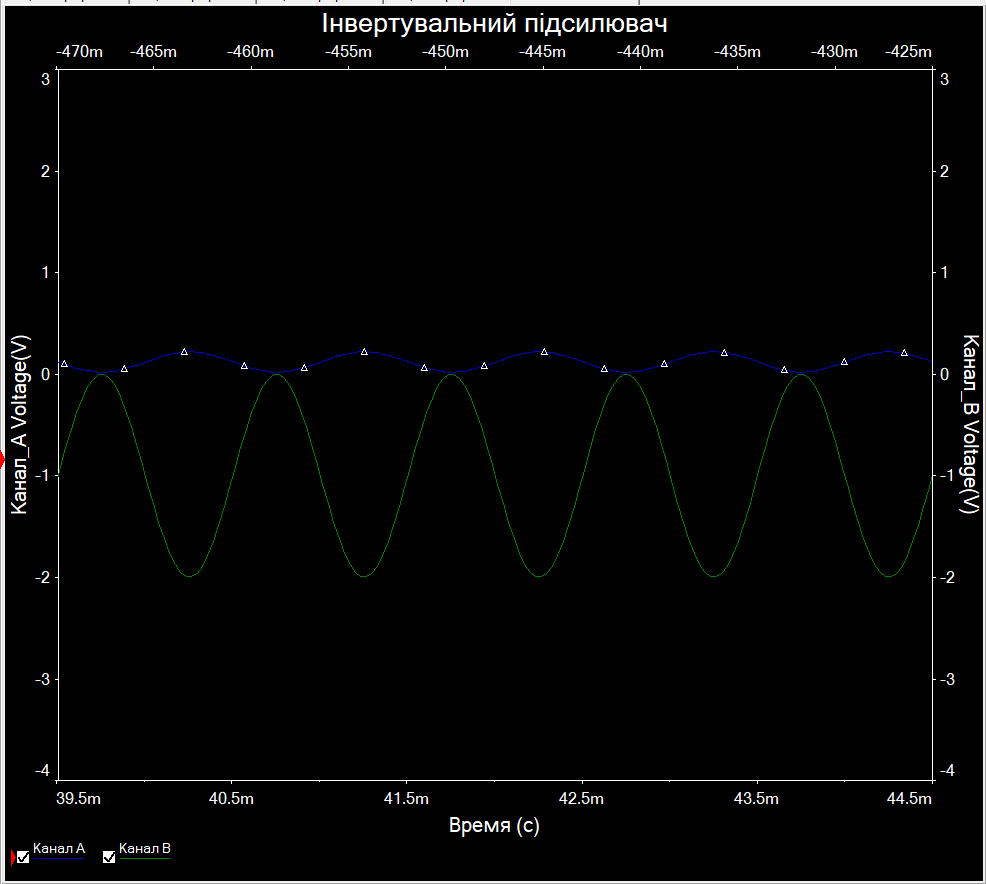
\includegraphics[width=0.6\textwidth]{imgs/1-2.png}
    \centering
    \caption{Залежність напруги на вході і виході від часу}
\end{figure}

\subsection{Неінвертувальний підсилювач}
\begin{figure}[H]
    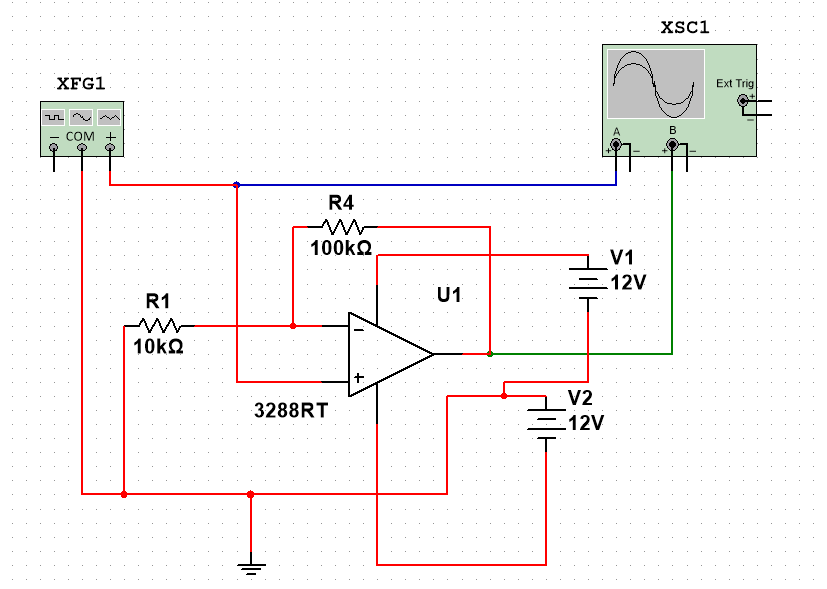
\includegraphics[width=0.6\textwidth]{imgs/2-1.png}
    \centering
    \caption{Схема}
\end{figure}
\begin{figure}[H]
    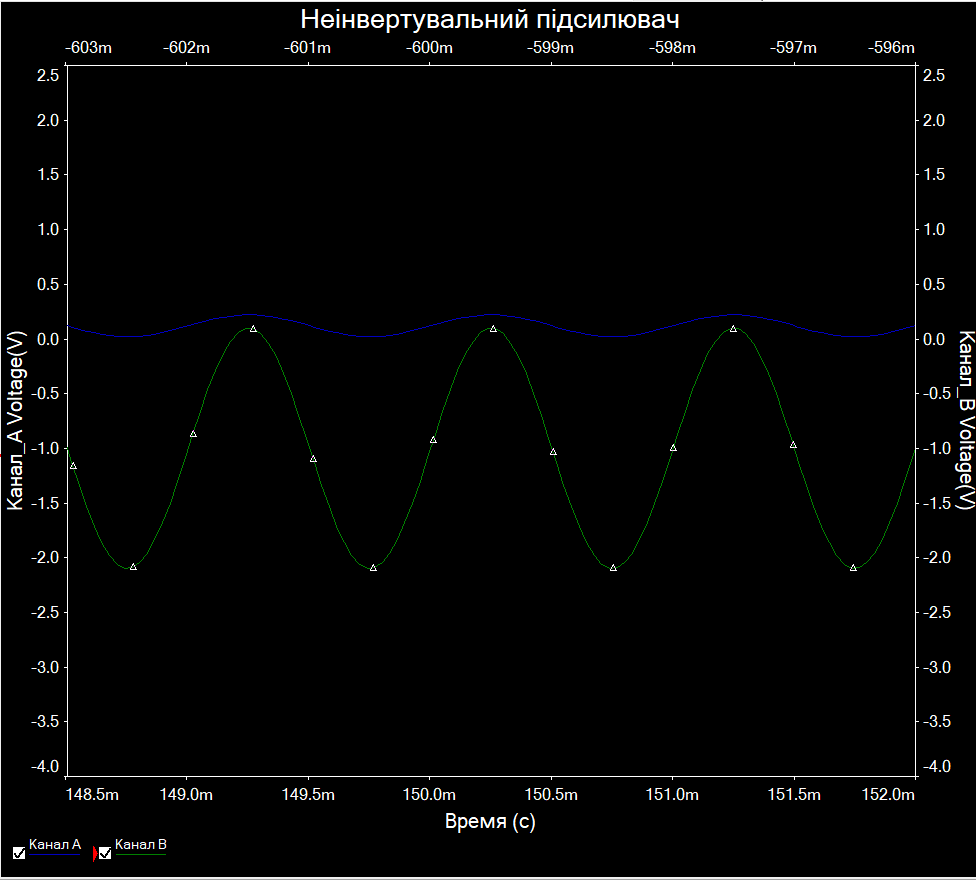
\includegraphics[width=0.6\textwidth]{imgs/2-2.png}
    \centering
    \caption{Залежність напруги на вході і виході від часу}
\end{figure}

\subsection{Інтегратор на базі інвертувального підсилювача}
\begin{figure}[H]
    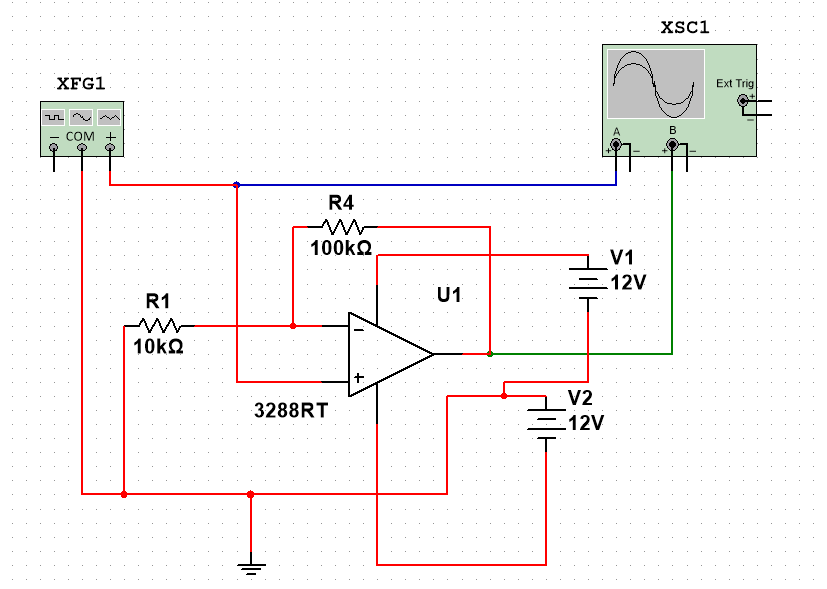
\includegraphics[width=0.6\textwidth]{imgs/2-1.png}
    \centering
    \caption{Схема}
\end{figure}
\begin{figure}[H]
    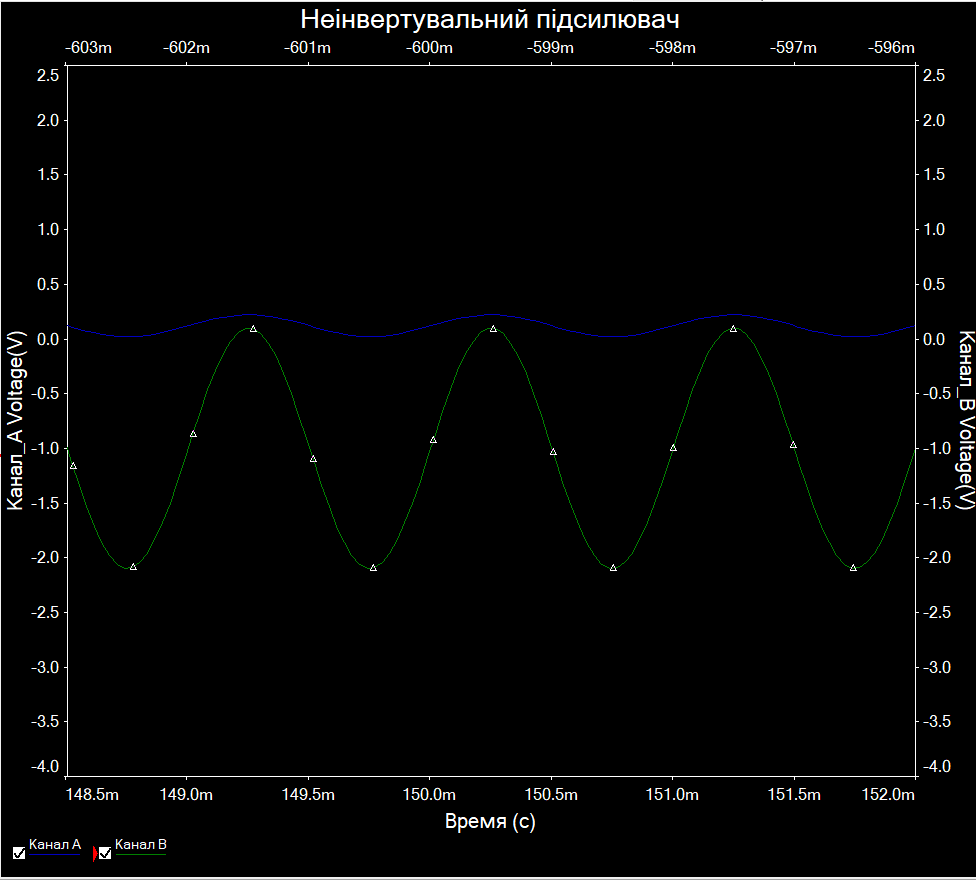
\includegraphics[width=0.6\textwidth]{imgs/2-2.png}
    \centering
    \caption{Залежність напруги на вході і виході від часу}
\end{figure}

\section{Висновок}
У даній лабораторній роботі вдалось дослідити ВАХ
операційних підсилювачів. При дослідження використовувались три типи ОП:
інтвертувальний, неінвертувальний підсилювач та інтегратор на базі
інвертувального підсилювача. Також познайомились із їхніми відмінностями. Для дослідження перших двох типів
використовувався гармонічний сигнал, для інтегратора — імпульсний.
Перевірили зміну фаз на вході та виході з кожного ОП. 

Робота виконувалась у програмі \textbf{Multisim14}.
\end{document}